\documentclass[twocolumn]{article}
\usepackage{verbatim}
\usepackage{amsfonts}
\usepackage{geometry}
\usepackage{amsmath}
\usepackage{amsthm}
\usepackage{amssymb}
\usepackage{listings}
\usepackage{graphicx}
\usepackage{clrscode3e}
\usepackage{txfonts}
\usepackage{fontspec}
\usepackage{float}
\usepackage{enumerate}
\setmainfont{Times New Roman}
\geometry{top=2.5cm,bottom=2.5cm,left=2.5cm,right=2.5cm}
\setlength\parindent{0em}
\begin{document}
	\title{Problem Solving Homework (Week 14)}\author{161180162 Xu Zhiming}\maketitle
	\section*{JH Chapter 2}
	\subsection*{2.2.3.21}
		\begin{figure}[H]
			\centering
			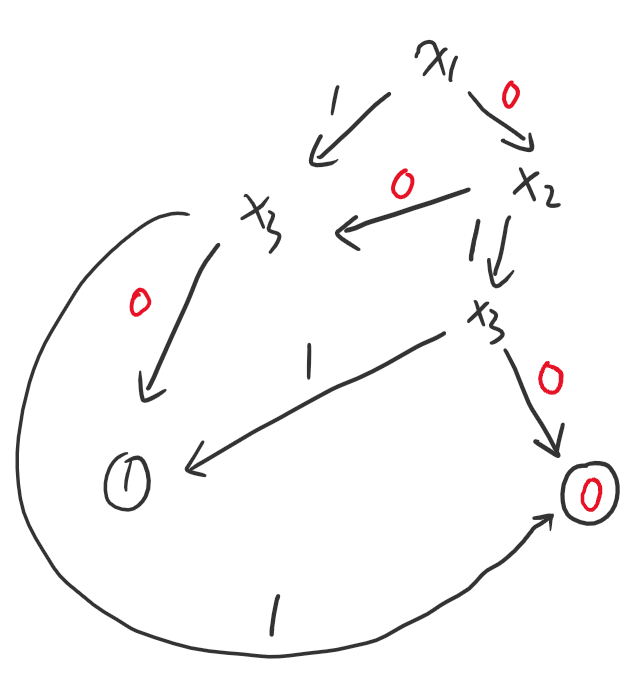
\includegraphics[width=0.7\linewidth]{hw14-1}
			\caption{The branching problem in (a) and (b) can be represented with the same graph}
		\end{figure}
		
	\subsection*{2.2.3.22}
	As is shown in the figure.
	\begin{figure}[H]
		\centering
		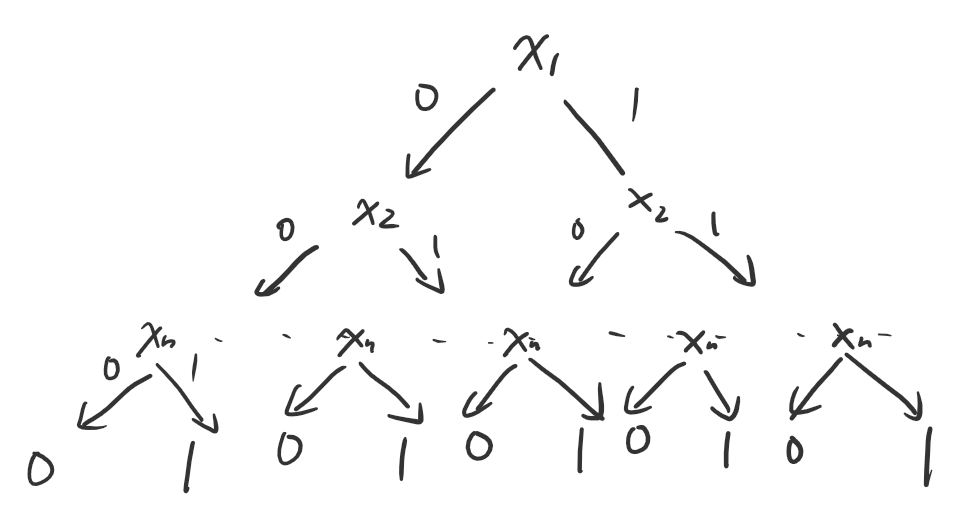
\includegraphics[width=1\linewidth]{hw14-2}
		\caption{For problem 22}
	\end{figure}
	\section*{JH Chapter 5}
	\subsection*{5.3.4.12}
	Since the main computation in \proc{Neq-Pol} comes from step 2 where two evaluations of polynomials are needed, we need to employ fast algorithm for that. Therefore, Horner's method is used for evaluation, which requires $d$ additions and $2d-1$ multiplication.
\end{document}